\section{一个有趣的应用:比较信息而不透露}\label{sec:4-8}

在这一节中,我们描述 PRF 的一个重要应用,称为\textbf{子密钥派生(sub-key derivation)}。假设 Alice 和 Bob 共享一个 PRF 的密钥 $k$。他们希望生成一连串的共享密钥 $k_1,k_2,\dots$,这样,他们就可以在不需要计算出所有之前的密钥的情况下计算出 $i$ 号密钥。当然,他们设置 $k_i:=F(k,i)$,其中 $F$ 是一个安全的 PRF,其输入空间为某个整数 $B$ 所约束的集合 $\{1,2,\dots,B\}$。

作为一个有趣的应用,考虑以下问题:Alice 在斯阔谷滑雪场度假,她想知道她的朋友 Bob 是否也在那里。如果他在的话,他们就可以一起滑雪。Alice 可以打电话问 Bob 他是否在滑雪场,但这将向 Bob 透露她在哪里,这是 Alice 不希望看到的。同样地,Bob 也很重视他的隐私,不想告诉 Alice 他在哪里,除非 Alice 刚好就在附近。

抽象地讲,这个问题可以表述如下:Alice 有一个数字 $a\in\mathbb{Z}_p$,Bob 也有一个数字 $b\in\mathbb{Z}_p$,其中,$p$ 为某个素数。这两个数字可以用来表示他们在地球上的大致位置。比如说,我们可以把地球表面分成 $p$ 块,而数字 $a$ 和 $b$ 就表示 Alice 和 Bob 目前在哪个块中。如果 Bob 也在滑雪场,那么 $a=b$,否则 $a\neq b$。

Alice 想知道 $a=b$ 是否成立;但是,如果 $a\neq b$,Alice 就不应该了解到关于 $b$ 的其他信息。同样,Bob 也不应该了解到关于 $a$ 的任何信息。

在之后的一章中,我们将看到如何确切地解决这个问题。在这里,我们先不妨假设 Alice 和 Bob 通过一个服务器 Sam 进行交互,这能使得问题变得简单一些。这个服务器会帮助 Alice 了解 $a=b$ 是否成立,但是它自己在这个过程中不会了解到什么信息。我们关于 Sam 的唯一假设是,它不与 Alice 或 Bob 串通,也就是说,它不会泄露 Alice 或 Bob 发送给它的隐私数据。显然,Alice 和 Bob 可以向 Sam 发送 $a$ 和 $b$,如果 $a=b$,它就会告诉 Alice 这一信息。但是,这样的话,Sam 就必须得知 $a$ 和 $b$,而我们的目标是让 Sam 什么都不知道,即使是在 $a=b$ 的情况下。

为了描述基本协议,我们假设 Alice 和 Bob 有共享一个密钥 $(k_0,k_1)\in\mathbb{Z}_p^2$。此外,Alice 和 Bob 各自与 Sam 构建了一条机密信道。那么,用于比较 $a$ 和 $b$ 的协议如图 \ref{fig:4-17} 所示。在协议开始时,Bob 从 $\mathbb{Z}_p$ 中随机选取一个 $r$,然后将 $(r,x_\mathrm{b})$ 发送给 Sam。Bob 可以随时进行这个操作,即使在 Alice 启动协议之前。当 Alice 想要比较两个整数时,她就将 $x_\mathrm{a}$ 也发送给 Sam。Sam 计算 $x\leftarrow rx_\mathrm{a}-x_\mathrm{b}$,然后将 $x$ 发回给 Alice。现在,注意到:
\[
x+k_1=r(a-b)
\]
所以,当 $a=b$ 时,我们有 $x+k_1=0$,否则,$x+k_1$ 有很大可能是非零的(假设 $p$ 足够大,所以 $r\neq0$ 的概率很大)。这就可以让 Alice 知晓 $a=b$ 是否成立。

\begin{figure}
  \centering
  

\tikzset{every picture/.style={line width=0.75pt}} %set default line width to 0.75pt        

\begin{tikzpicture}[x=0.75pt,y=0.75pt,yscale=-1,xscale=1]
%uncomment if require: \path (0,138); %set diagram left start at 0, and has height of 138

%Straight Lines [id:da8062637216156805] 
\draw[->]    (70,80) -- (270,80) ;
%Straight Lines [id:da31337861884224827] 
\draw[<-]    (70,110) -- (270,110) ;
%Straight Lines [id:da9857458477267009] 
\draw[->]    (310,70) -- (510,70) ;

% Text Node
\draw (2,3) node [anchor=north west][inner sep=0.75pt]   [align=left] {Alice};
% Text Node
\draw (2,23) node [anchor=north west][inner sep=0.75pt]   [align=left] {input: $\displaystyle a$};
% Text Node
\draw (170,76.6) node [anchor=south] [inner sep=0.75pt]    {$x_{\mathrm{a}}\leftarrow a+k_{0}$};
% Text Node
\draw (170,106.6) node [anchor=south] [inner sep=0.75pt]    {$x\leftarrow rx_{\mathrm{a}} -x_{\mathrm{b}}$};
% Text Node
\draw (2,110.05) node [anchor=west] [inner sep=0.75pt]    {$x+k_{1}\overset{?}{=} 0$};
% Text Node
\draw (410,66.6) node [anchor=south] [inner sep=0.75pt]    {$r,\ \ \ x_{\mathrm{b}}\leftarrow r( b+k_{0}) +k_{1}$};
% Text Node
\draw (545,71.6) node [anchor=south] [inner sep=0.75pt]    {$r\overset{\mathrm{R}}{\leftarrow }\mathbb{Z}_{p}$};
% Text Node
\draw (290,3) node [anchor=north] [inner sep=0.75pt]   [align=left] {Server};
% Text Node
\draw (290,23) node [anchor=north] [inner sep=0.75pt]   [align=left] {Sam};
% Text Node
\draw (522,3) node [anchor=north west][inner sep=0.75pt]   [align=left] {Bob};
% Text Node
\draw (522,23) node [anchor=north west][inner sep=0.75pt]   [align=left] {input: $\displaystyle b$};


\end{tikzpicture}
  \caption{在不透露 $a$ 和 $b$ 的情况下比较它们}
  \label{fig:4-17}
\end{figure}

这个协议会披露什么信息?很明显,Bob 什么信息都没有得到。Alice 知道了 $r(a-b)$,但如果 $a\neq b$,这就是一个均匀分布在 $\mathbb{Z}_p$ 上的值。因此,当 $a\neq b$时,Alice 只是获得了一个均匀分布在 $\mathbb{Z}_p$ 上的元素,除了 $a\neq b$ 这个事实之外,这没有透露任何信息。Sam 看到了 $r$,$x_\mathrm{a}$ 和 $x_\mathrm{b}$,但这三个值都与 $a$ 和 $b$ 无关:$x_a$ 和 $x_b$ 分别是使用密钥 $k_0$ 和 $k_1$ 在一次性密码本下的加密。因此,Sam 也什么都没学到。请注意,关于 Sam 的唯一隐私假设是它不向 Alice 透露 $(r,x_\mathrm{b})$ 或向 Bob 透露 $x_\mathrm{a}$。

\vspace{8pt}

问题在于,和一次性密码本一样,共享密钥 $(k_0,k_1)$ 只能用于\emph{一次}相等测试中,否则协议就不安全了。如果 $(k_0,k_1)$ 被用来测试$a=b$ 是否成立,之后又被用来测试 $a'=b'$ 是否成立,那么 Alice 和 Sam 就能够知道他们本不应该知道的信息。此外,Alice 还可以推导出 $(a-b)/(a'-b')$,这就揭示了关于 $b$ 和 $b'$ 的信息(例如,如果 $a=a'=0$,那么 Alice 就会知道 $b$ 和 $b'$ 的比例)。

\begin{snote}[子密钥的派生。]
那么,如果 Alice 想反复测试与 Bob 的接近程度怎么办?解决方案是,为协议的每次调用都生成一个新的独立密钥 $(k_0,k_1)$。我们可以使用一个安全的 PRF 来派生针对特定实例的子密钥。

令 $F$ 是一个定义在 $(\mathcal{K},\{1,\dots,B\},\mathbb{Z}^2_p)$ 上的一个安全的 PRF,并假设 Alice 和 Bob 共享一个长期密钥 $k\in\mathcal{K}$。Bob 维护一个计数器 $cnt_\mathrm{b}$,它最初被置为 $0$。每当 Bob 向 Sam 发送他的加密位置 $(r,x_\mathrm{b})$ 时,他都会将 $cnt_\mathrm{b}$ 递增,并从长期密钥 $k$ 中推导出子密钥 $(k_0,k_1)$,方法是:
\begin{equation}\label{eq:4-46}
(k_0,k_1)\leftarrow F(k,cnt_\mathrm{b})
\end{equation}
他把 $(r,x_\mathrm{b},cnt_\mathrm{b})$ 发送给 Sam。Bob 可以随时这样做,比如说每隔几分钟,或者每当他移动到一个新的地点时。

每当 Alice 想测试与 Bob 的接近程度时,她首先要求 Sam 向她发送来自 Bob 的最新消息中计数器的值。她要确保这个计数器值比 Sam 发给她的前一个值要大(以防止调皮的 Sam 或 Bob 通过复用一个旧的计数器值来欺骗 Alice)。然后 Alice 自己用式 \ref{eq:4-46} 计算 $(k_0,k_1)$,并使用这些密钥执行图 \ref{fig:4-17} 中与 Sam 的协议。

由于 $F$ 是一个安全的 PRF,所以派生出的子密钥序列与独立采样的随机密钥是不可区分的。这就保证了重复的协议除了相等关系之外不会透露任何关于测试值的信息。通过使用 PRF,Alice 就能够快速计算出对于最新的 $cnt_\mathrm{b}$ 的密钥 $(k_0,k_1)$。
\end{snote}